\documentclass[11pt]{book}
\usepackage{gvv-book}
\usepackage{gvv}

\usepackage{caption} % Add the caption package

\begin{document}

\section{NCERT 12.10.5.9}

Find the position vector of a point $\vec{R}$ which divides the line joining two points $\vec{P}$ and $\vec{Q}$ whose Position Vectors are $2\vec{a}+\vec{b}$ and $\vec{a}-3\vec{b}$ externally in the ratio $1:2$. \\
\textbf{Solution:}
let us assume $\vec{a}$ and $\vec{b}$ and the given ratio is
\begin{table}[H]
\begin{center}
 \begin{tabular}{|c|c|c|}
	 \hline 
        \textbf{Symbol} & \textbf{Value} & \textbf{Description} \\
        \hline
	    $\vec{a}$ & $\myvec{1 \\ -3}$ & vector $\vec{a}$ \\
        \hline
	    $\vec{b}$ & $\myvec{0 \\ 2}$ & vector $\vec{b}$\\
        \hline
        $k$ & $2$ & ratio \\
        \hline
    \end{tabular}
    \end{center}
    \captionsetup{justification=centering} % Center the table caption
    \caption{Vectors $\vec{a}$ and $\vec{b}$, ratio $k$}
    \label{tab:table1}
\end{table}

using section formula
\begin{align}
    \vec{R}=\frac{\vec{Q}-k.\vec{P}}{1-k}
\end{align}\\
where $\vec{P}$ and $\vec{Q}$ depends on $\vec{a}$ and $\vec{b}$ then,
\begin{align}
	\vec{P}=(2\vec{a}+\vec{b})=2\myvec{1\\-3}+\myvec{0\\2}=\myvec{2\\-4}\\
    \vec{Q}=(\vec{a}-3\vec{b})=\myvec{1\\-3}-3\myvec{0\\2}=\myvec{1\\-9}
\end{align}\\
where $\vec{R}$ can be calculated as 
\begin{align}
	\vec{R}=\frac{(\vec{a}-3\vec{b})-k.(2\vec{a}+\vec{b})}{1-k}
\end{align}\\
by substituting $\vec{a}$ and $\vec{b}$ values we get $\vec{R}$ as
\begin{align}
    \vec{R}=\myvec{3\\1}
\end{align}
\centering
\begin{table}[H]
    \begin{center}
         \begin{tabular}{|c|c|c|}
        \hline
        \textbf{Symbol} & \textbf{Value} & \textbf{Description}\\
        \hline
	    $\vec{P}$ & $(2\vec{a}+\vec{b})$ & position vector $\vec{P}$ \\
        \hline
	    $\vec{Q}$ & $(\vec{a}-3\vec{b})$ & position vector $\vec{Q}$\\
        \hline
	    $\vec{R}$ & $\frac{\vec{Q}-k.(\vec{P})}{1-k}$ & position vector $\vec{R}$\\
        \hline
    \end{tabular}
    \end{center}
    \captionsetup{justification=centering} % Center the table caption
    \caption{Vectors $\vec{P}$, $\vec{Q}$, $\vec{R}$}
    \label{tab:mytable2}   
\end{table}

\begin{figure}[!ht]
    \centering
    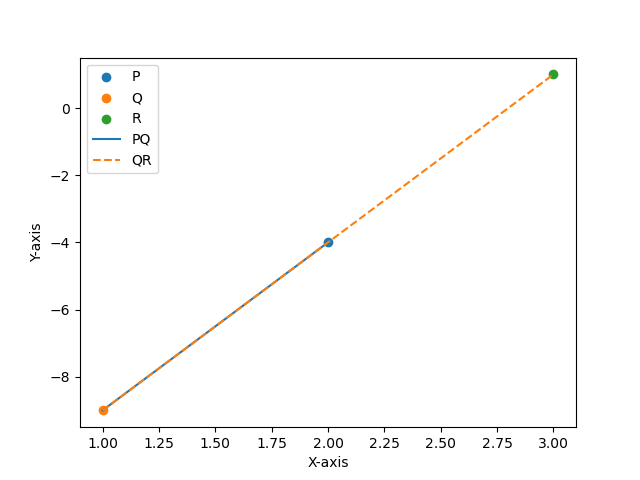
\includegraphics[width=\columnwidth]{/home/ramsai/MathComputing/codes/python/external-bisector.png}
    \captionsetup{justification=centering} % Center the figure caption
    \caption{Point vectors $\vec{P}$, $\vec{Q}$, $\vec{R}$}
    \label{fig:enter-label}
\end{figure}
\end{document}

